\newpage
\section{CFD Model}
\subsection{Simulation parameters}
\label{subsec:simulation_parameters}

\subsubsection{Solver settings}

The simulation is made with SolidWorks Flow Simulation. It use an implicit solver based on finit volumses (FVM). The solver is CFD NIKA which is a commercial solver create by Dassault Systems. It's base on a 3d flow Navier-Stocks equations with a turbulent model $k-\epsilon$ and conjugate heat transfer (CHT).

\subsubsection{Geometry}

The flow on a slope is depending only of two dimensions. So the problem is reduced to only two varialb the slope $\theta$ and the Mach number $M$. So that the solution is $\beta = f(\theta,M)$.

\begin{figure}[H]
    \centering
    \begin{minipage}[b]{0.45\linewidth}
        \centering
        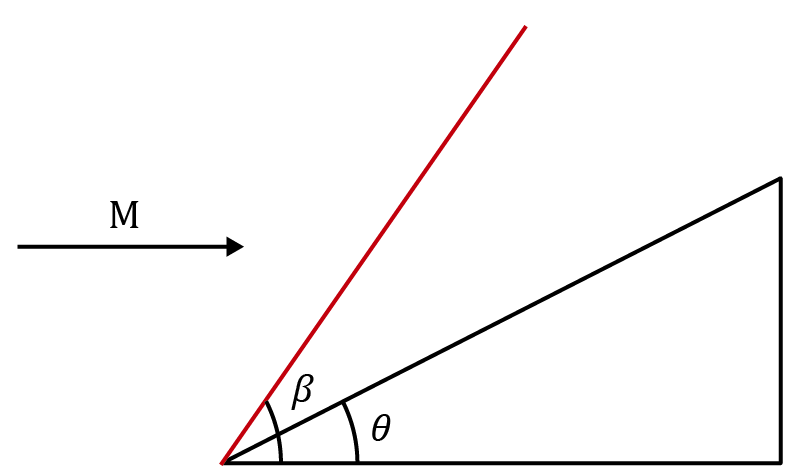
\includegraphics[width=\linewidth]{ressources/images/Slope.png}
		\caption{Geometry}
    \end{minipage}
    \begin{minipage}[b]{0.45\linewidth}
        \centering
        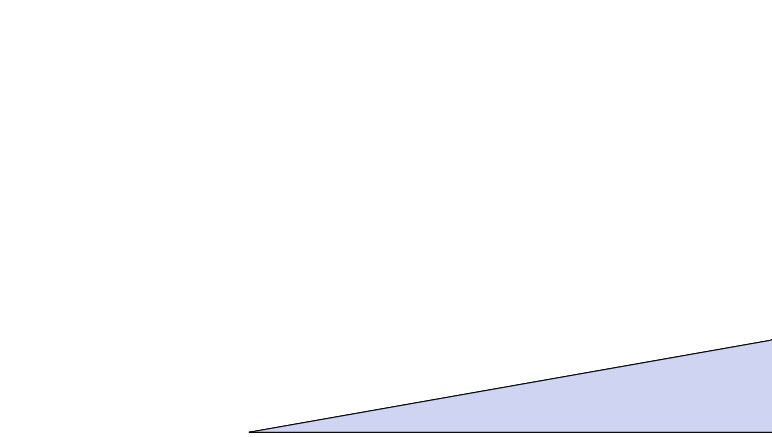
\includegraphics[width=\linewidth]{ressources/images/SlopeSW.jpg}
		\caption{SolidWorks View}
    \end{minipage}
    \label{fig:slope}
\end{figure}

The fix variable of the geometry is here the length of the triangle fix at $50cm$.

\subsubsection{Mesh}
For the problem we can use a 2D mesh with a refinement that progress logaritmically whith the distance. At the largest part of the grid there is a point evry $0.0881cm$ and at the thinest part of the grid $0.0042cm$.
\begin{figure}[H]
	\centering
	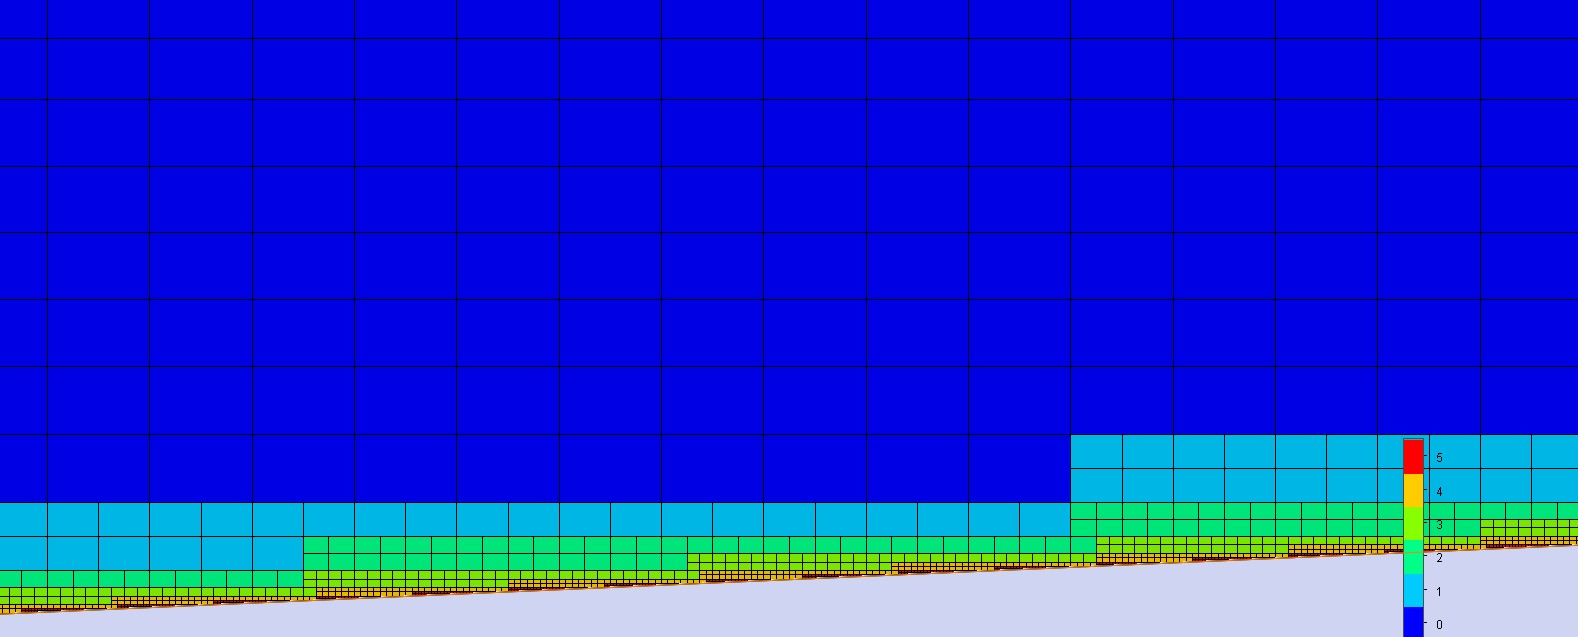
\includegraphics[width=0.8\linewidth]{ressources/images/CFD/Maillage.jpg}
	\caption{Mesh}
	\label{fig:mesh}
\end{figure}


\subsection{Simulation}

\subsubsection{Resutls}
In the objective to get the shock angle $\beta$ the best solution is to compute the pressure in evry points. So the shock wave will be place where there is a pressure drop line, then compute the angle between this line and the x axe.
To do the simulation run until a flow-mas convergent solution is found.

\begin{figure}[H]
	\centering
	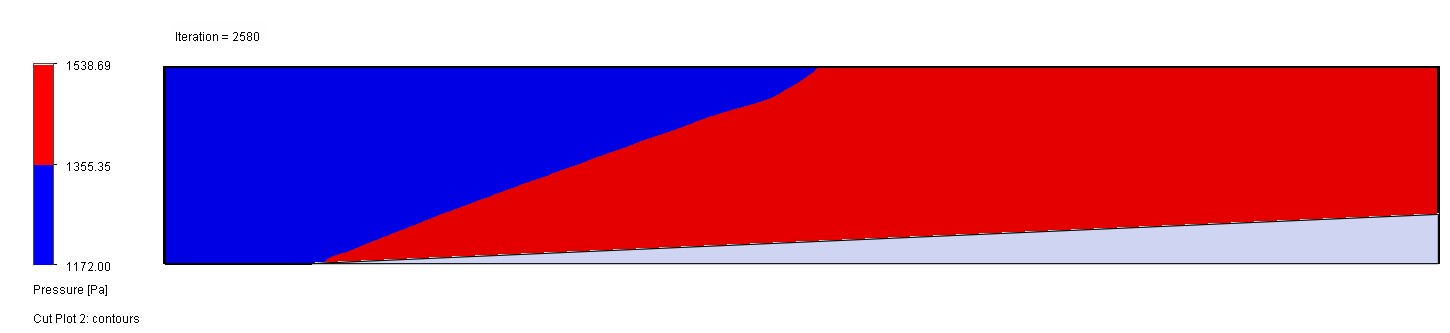
\includegraphics[width=0.8\linewidth]{ressources/images/CFD/SolidWorks1.jpg}
	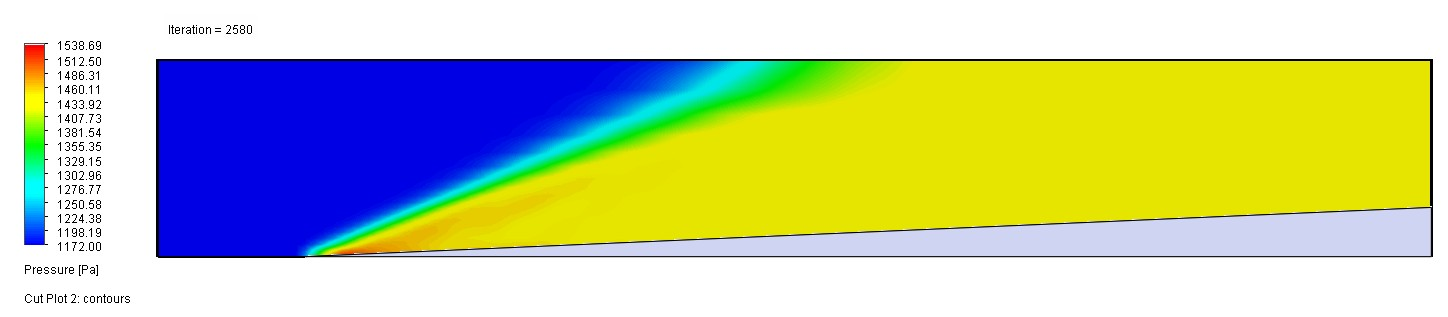
\includegraphics[width=0.8\linewidth]{ressources/images/CFD/SolidWorks2.jpg}
	\caption{SolidWorks Pressure Results}
	\label{fig:resSW}
\end{figure}

\subsubsection{Exportation}
To be able to analys the results it is needed to export them out of SolidWorks because we can't apply algorithm to find the shock angle inside. \\
The exportation are on the .txt format wich is hard to read so it was important to convert this into .csv. On top of that it's important to make sure that the varaible are as following

\begin{pycode}
lines[0] = 'X [m] Y [m] Z [m] Volume [m^3] Pressure [Pa]\n'
\end{pycode}



\subsection{Results analysis}

\subsubsection{$1^{st}$ Visualization}
To make sure that we are working on the right dataset and also to plot later the result on the pressure chart. It is important first to see the data inside python, trough matplotlib here.

\begin{figure}[H]
	\centering
	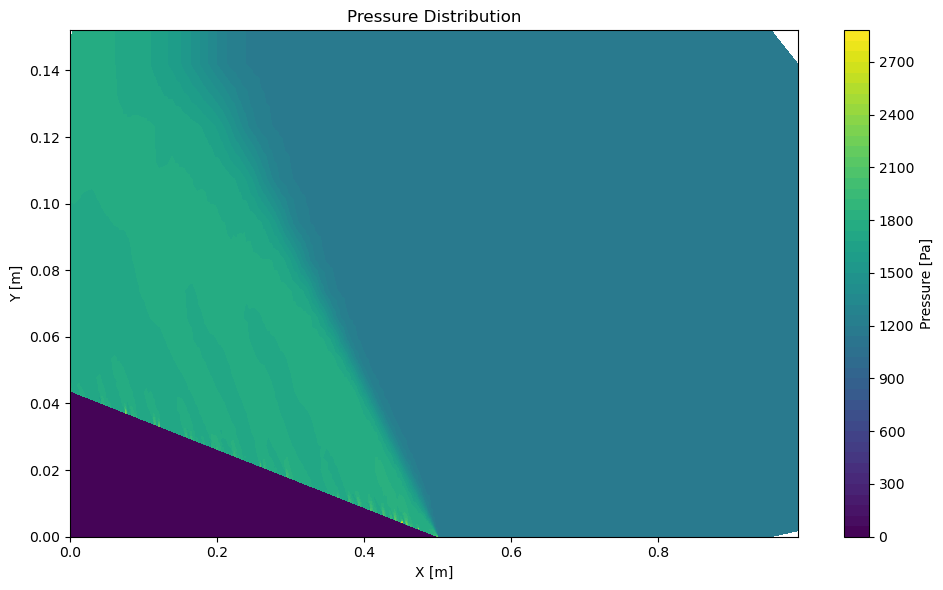
\includegraphics[width=0.5\linewidth]{ressources/figures/PressureDistribution.png}
	\caption{$1^{st}$Visualization}
	\label{fig:resSW}
\end{figure}

As expected we have 3 pressure zone in the dataset. One before the shock, one after the shock a not a real on insinde the geometry where the pressure is 0 because it's inside the solide.

\subsubsection{K-Means}
To manage to find the three pressure zones explained before — the region before the shock, the region after the shock, and the interior of the solid — we use an unsupervised machine learning algorithm called K-Means.

K-Means is a clustering algorithm that partitions a set of data points into a predefined number of clusters (in our case, $k=3$). The goal is to group the data so that points within each cluster are as close as possible to the cluster center (centroid), while being as far as possible from the centers of the other clusters.

Once clustered, we can export the points that compose the borders and plot them.

\begin{figure}[H]
	\centering
	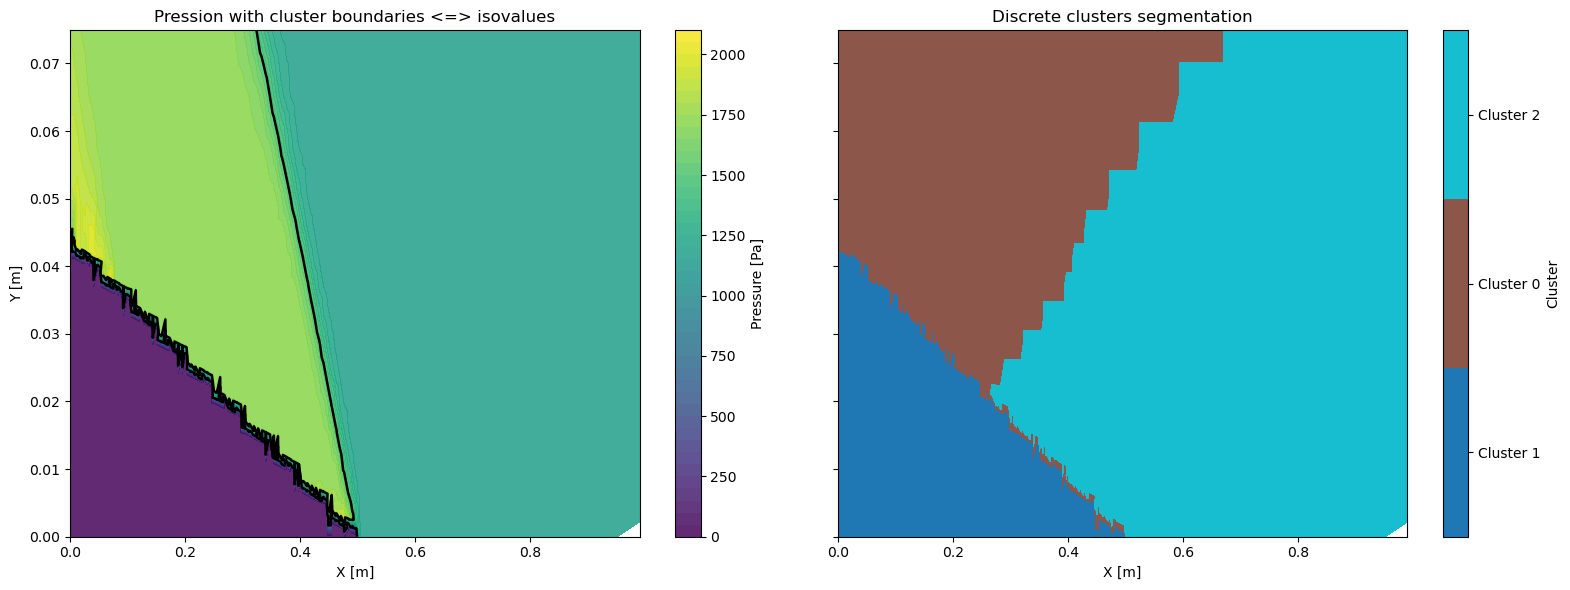
\includegraphics[width=0.8\linewidth]{ressources/figures/Kmeans.png}
	\caption{Clustering}
	\label{fig:clustering}
\end{figure}


\subsubsection{Interpetation}

Now it is possible to do some linear approximation on the borders to get draw some slopes.

\begin{figure}[H]
	\centering
	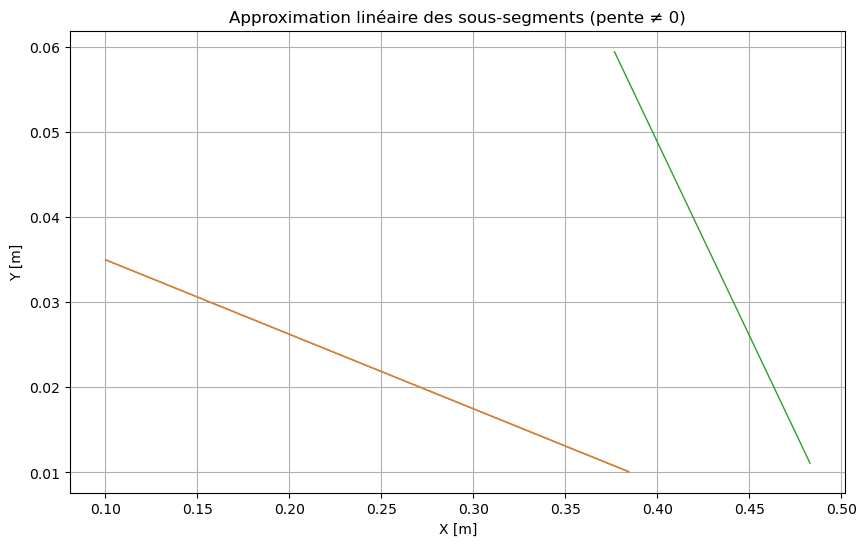
\includegraphics[width=0.5\linewidth]{ressources/figures/slope.png}
	\caption{Slopes}
	\label{fig:slopes}
\end{figure}

With this slopes it is possible to reject the one with the smallest variation. Only to conserve the shock one and then compute the angle base on the slope, wich give the following result.

\begin{figure}[H]
	\centering
	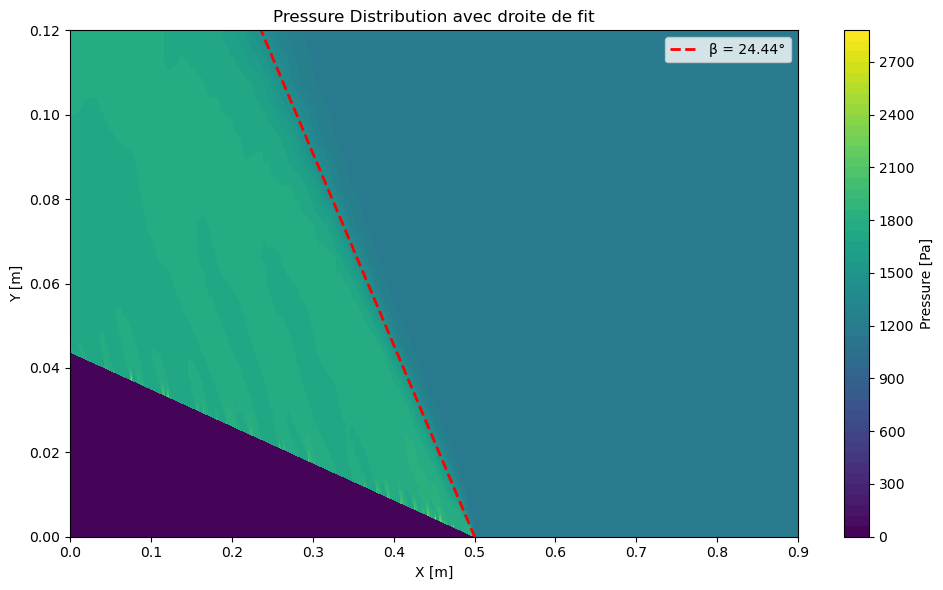
\includegraphics[width=0.5\linewidth]{ressources/figures/final_slope.png}
	\caption{Simulation Interpetation}
	\label{fig:interpetation}
\end{figure}


\subsubsection{Repetition}
With the geometry parameters and the process to analys the result it is possible to duplicate the simulations to compare with the theoritical values.

\begin{figure}[H]
    \centering
    \begin{minipage}[b]{0.45\linewidth}
        \centering
		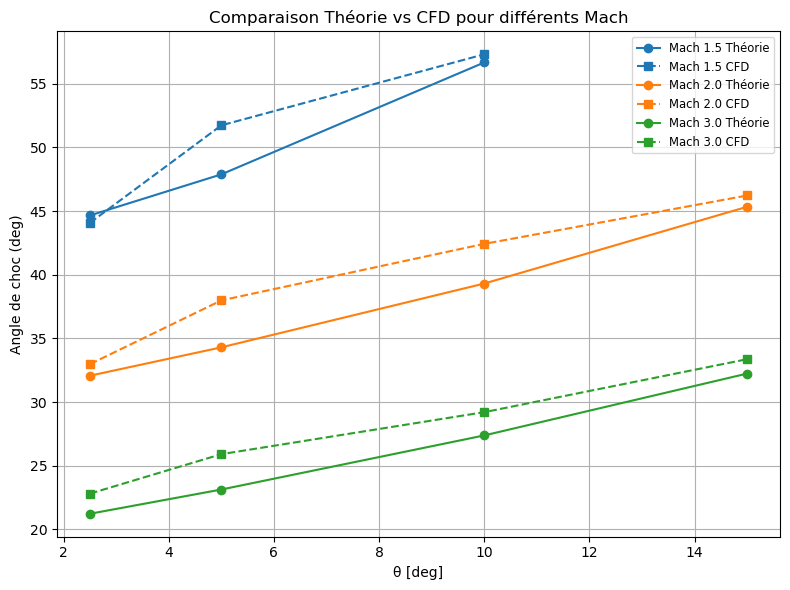
\includegraphics[width=1\linewidth]{ressources/figures/sol1.png}
    \end{minipage}
    \begin{minipage}[b]{0.45\linewidth}
        \centering
		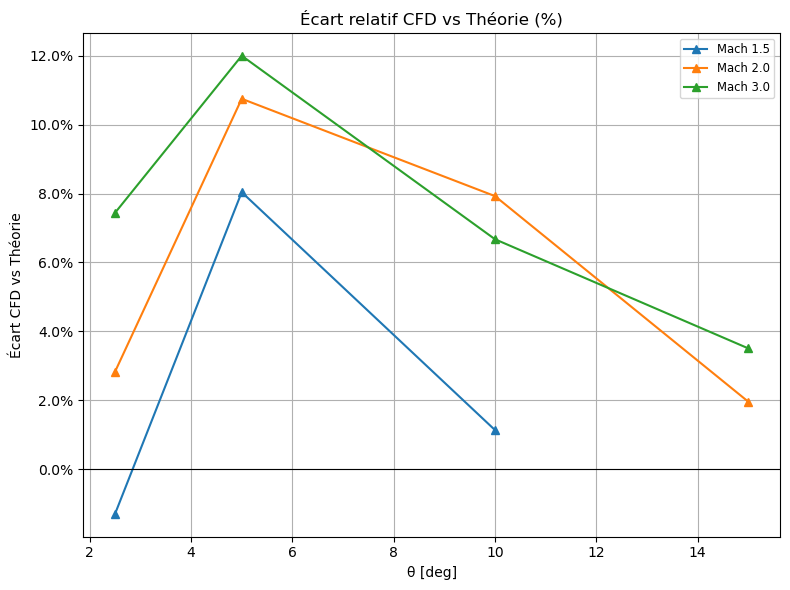
\includegraphics[width=1\linewidth]{ressources/figures/sol2.png}
    \end{minipage}
	\caption{Solution comparaison}
    \label{fig:sol}
\end{figure}

We can see the error is never over 12\% so it is clear that the simulation feat well with the theory. This error is probably mainly due to the hypothesis of infinitesimal thickness in the theory.
